\section{Anforderungen und Herausforderungen}
\sectionmark{Anf} % short form for headlines on pages
% Gedankengang beschreiben
% Wie sind wir zur Lösung gekommen?
% Herausforderungen und Probleme nennen
Um Kollisionen mit anderen Duckiebots zu vermeiden, wurde eine Node entwickelt, die auf Basis des, am Duckiebot eingebauten, ToF-Sensors (Time of Flight) arbeitet. Diese Node ist dafür verantwortlich, den Abstand zu anderen Robotern zu messen und gegebenenfalls eine Korrektur der Fahrtrichtung bzw. der Fahrtgeschwindigkeit vorzunehmen.

Eine zentrale Herausforderung bestand darin, zuverlässige Abstandsmessungen in Echtzeit zu gewährleisten, da der ToF-Sensor durch Umgebungslicht, reflektierende Oberflächen und die Bewegung des Roboters beeinflusst werden kann. Außerdem musste die Hardware am Duckiebot überprüft werden, dass zuverlässige Daten gesendet werden. Die Node wurde so gestaltet, dass sie schnell genug auf erkannte Hindernisse reagiert, um eine Kollision sicher zu vermeiden, ohne dabei unnötig oft oder abrupt zu bremsen.

Ein weiteres Problem war die Integration der Node in das bestehende Steuerungssystem des Duckiebots, sodass die Kollisionsvermeidung nahtlos mit anderen Fahrfunktionen zusammenarbeitet. Hierbei mussten Prioritäten zwischen verschiedenen Steuerbefehlen festgelegt und getestet werden, um ein sicheres und flüssiges Fahrverhalten zu gewährleisten.




\section{Ablaufdiagramm}
\sectionmark{Impl} % short form for headlines on pages
% Ablaufdiagramm und Beschreibung der Node
\begin{figure}[H]
    \centering
    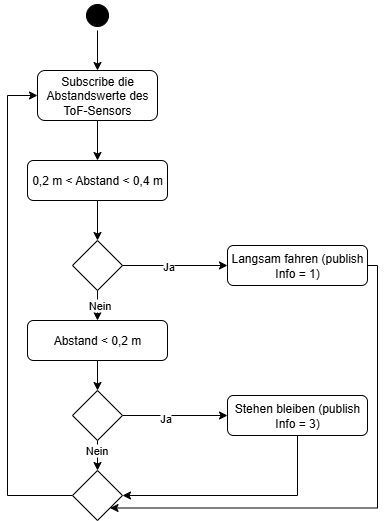
\includegraphics[width=0.8\textwidth]{Figures/png/Ablaufdiagramme_Bericht-Collision_Avoidance.drawio.png}
    \caption{Ablaufdiagramm der Collision Avoidance Node}
    \label{fig:collision_avoidance_node}

\end{figure}
In Abbildung \ref{fig:collision_avoidance_node} ist das Ablaufdiagramm der Collision Avoidance Node dargestellt. Die Node beginnt mit der Initialisierung der Sensoren und der ROS-Kommunikation. Anschließend wird in einer Endlosschleife kontinuierlich der Abstand zu Hindernissen vor dem Sensor gemessen. Wenn ein Hindernis in einem Bereich von 0,2 m bis 0,4 m erkannt wird, wird die Fahrtgeschwindigkeit reduziert, um das Hindernis langsam anzufahren. Kommt das Hindernis näher als 0,2 m hält der Duckiebot an, um eine Kollision zu vermeiden. Nach der Anpassung der Geschwindigkeit überwacht die Node weiterhin den Abstand um weiterfahren zu können, wenn das Hindernis nicht mehr im kritischen Erfassungsbereich ist.

\section{Technische Umsetzung im Code}
\sectionmark{Tech} % short form for headlines on pages
% Beschreibung wie man es im Code umgesetzt hat
Die Node subscribed die Abstandswerte des ToF-Sensor und verarbeitet diese in der Callback-Funktion. In einer run-Funktion wird der Abstandswert kontinuierlich überwacht und entsprechende Aktionen ausgelöst, wenn die definierten Schwellenwerte überschritten oder unterschritten werden. Die Node published den aktuellen Betriebsmodus des Duckiebots – „langsam“ oder „stop“ – zur weiteren Verarbeitung.
Erkennt die Node kein Hindernis, wird keine Information veröffentlicht, sodass die Steuerungs-Node den Duckiebot mit voller Geschwindigkeit im Spurverfolgungsmodus weiterfahren lässt.

%% End of File %%